%!TEX root = ../my_thesis.tex
\chapter{Décodeurs polaires déclenchés par transport} % (fold)
\label{chap:tta}

\vspace*{\fill}
\minitocTITI
\vspace*{\fill}
\newpage

\section*{Introduction}



\section{Transport Triggered Architectures}


\subsection{Principes}

Au cours de ce manuscrit, du point de vue de l'architecture des processeurs, deux types de parallélisme ont été abordés.
Le premier est le parallélisme de données.
Pour exploiter ce parallélisme, les jeux d'instructions de certains processeurs incluent des instructions vectorielles SIMD.
C'est le cas des architectures ARM ou x86 actuelles qui incluent respectivement les jeux d'instructions NEON et AVX utilisés dans le Chapitre \ref{chap:soft_scl}.
Les instructions spécialisées de l'ASIP proposé dans le Chapitre \ref{chap:tensilica} sont également des instructions SIMD.
Ces instructions permettent d'appliquer parallèlement une même opération sur plusieurs données.

Le second type de parallélisme est le parallélisme d'instructions. Contrairement au parallélisme de données, il s'agit d'exécuter plusieurs opérations différentes sur plusieurs données d'entrées. Par exemple, effectuer une somme de deux données et, en parallèle, effectuer une opération \textit{ou-exclusif} sur deux autres.
Il existe plusieurs façons de concevoir un processeur permettant du parallélisme d'instructions. Le compilateur peut selon les cas être impliqué dans la détection et l'exploitation du parallélisme d'instructions.

Dans les architecture superscalaires, le compilateur n'est pas impliqué dans la gestion du parallélisme d'instructions. Celui-ci est détecté par des unités matérielles spécialisées. 
Elles permettent de lancer l'exécution de plusieurs opérations parallèles sur les multiples unités fonctionnelles du processeur.
Pour cela, ces unités ont la capacité d'analyser les dépendances entre les données, de changer dynamiquement l'ordre d'exécution des instructions, ainsi que de spéculer sur les futures instructions du programme exécuté. 
Un des avantages de ce type de processeurs est que des programmes séquentiels d'architectures plus anciennes peuvent être accélérés dans nouvelle compilation. Le désavantage est le complexité accrue du processeur causée par l'ajout des unités matérielles responsables de la mise en œuvre du parallélisme. La surface du circuit augmente ainsi que sa consommation énergétique.

Au contraire, dans les architectures dites \og à très long mot d'instruction \fg (VLIW : Very Large Instruction Word), l'essentiel de l'effort nécessaire à la mise en œuvre du parallélisme d'instructions est pris en charge par le compilateur. Le compilateur décrit quelles instructions doivent être exécutées en parallèle, et dans quel ordre. L'avantage des architectures VLIW par rapport aux architectures superscalaires est la réduction de la complexité de la logique de contrôle. De plus, les possibilité de parallélisme d'instructions sont plus facilement identifiées par les compilateurs qui ont une vue plus large du programme que les unités matérielles de parallélisation des architectures superscalaires.


\begin{figure}[htp]
\centering
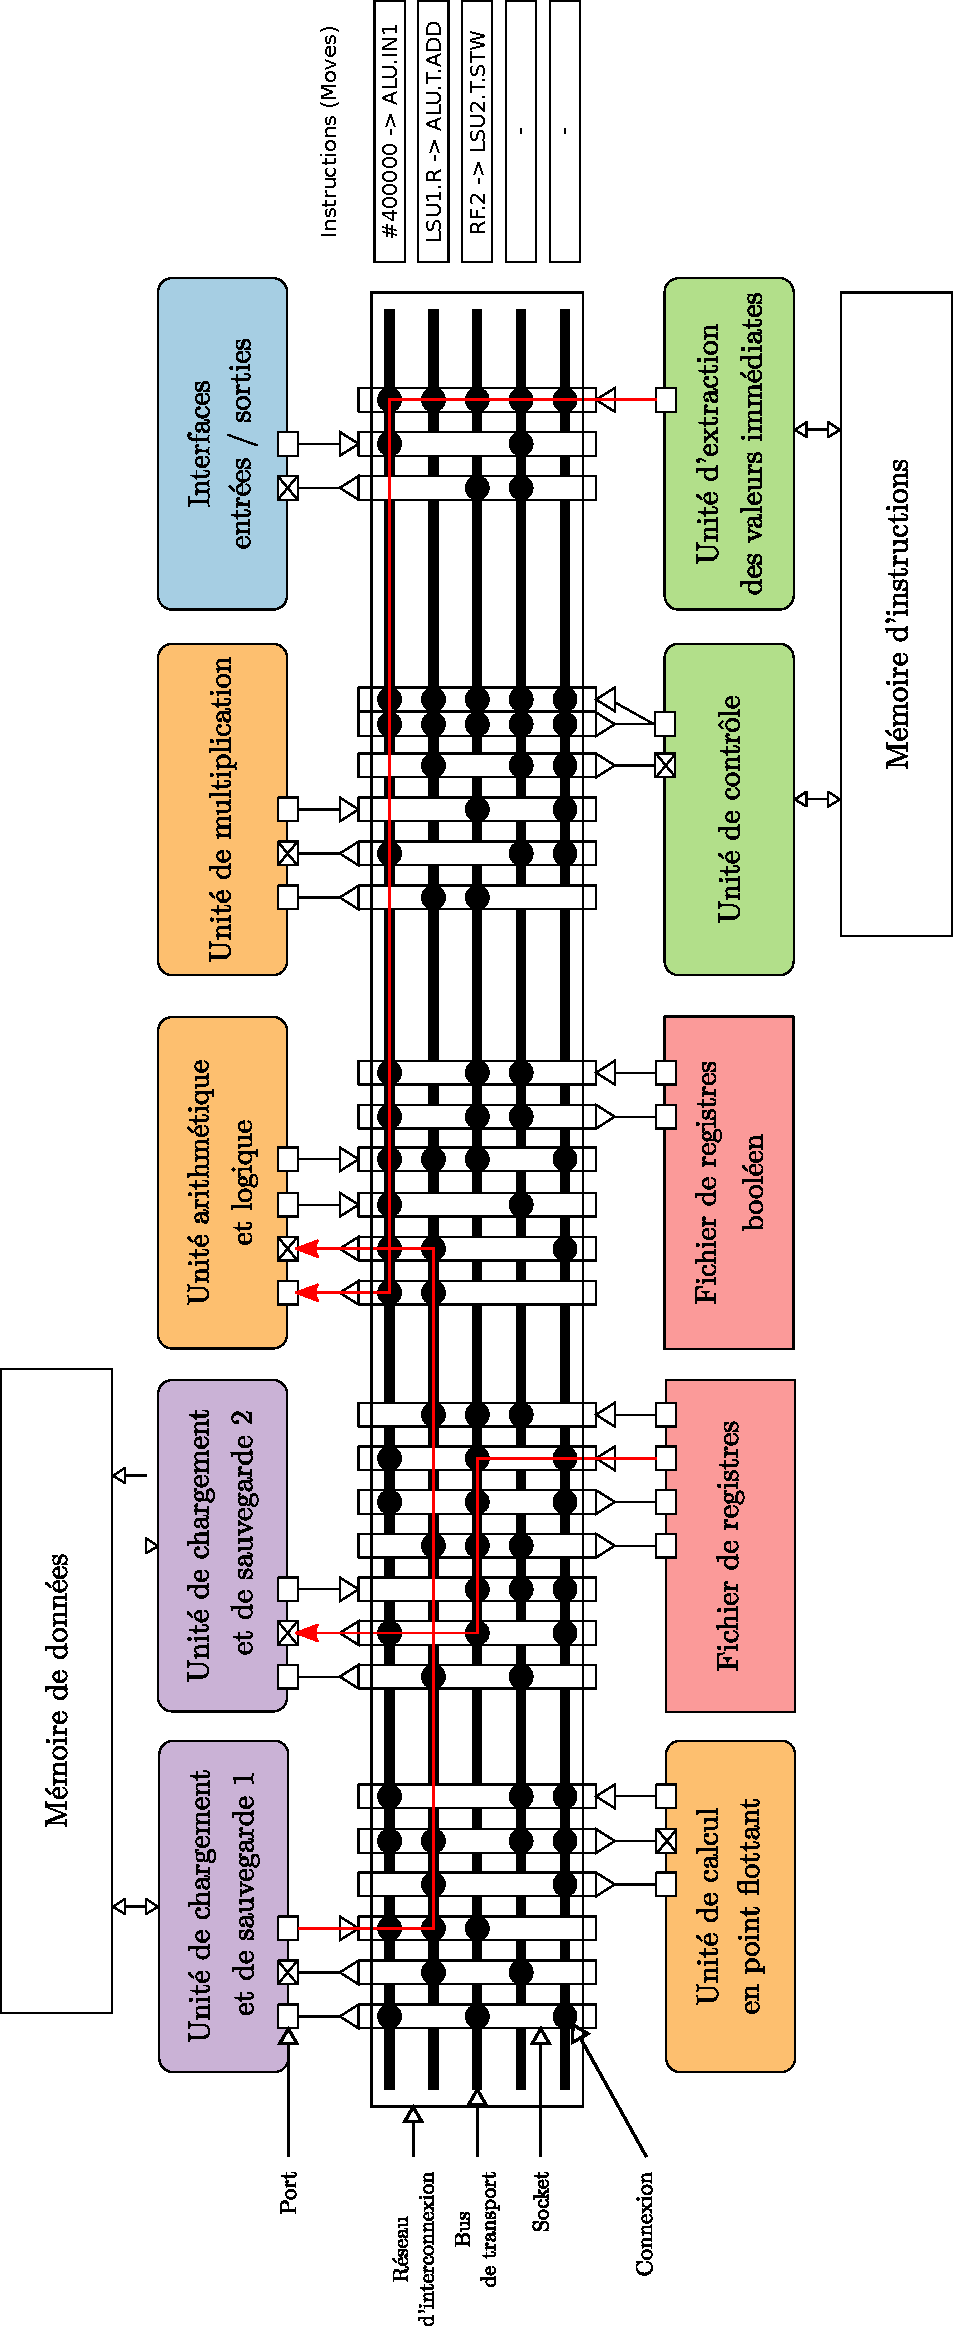
\includegraphics[width=\textwidth]{main/ch4_fig/archi_tta}
\caption{Un exemple d'architecture de processeur TTA.}
\label{fig:tta_example}
\end{figure}

L'architecture du processeur proposé dans ce chapitre fait partie de la famille des architectures déclenchées par le transport (TTA : Transport Triggered Architecture). Les TTAs sont des architectures modulaires particulières proches des architectures VLIW. La Figure \ref{fig:tta_example} présente un exemple d'architecture TTA \cite{pekka_phd_2012} Au centre, on trouve les \textit{bus de transport} sur lesquels les données transitent. Sur ces bus de transport sont connectées les \textit{unités fonctionnelles}, par l'intermédiaire des \textit{socket} et des \textit{ports}. Les \textit{ports} font partie des \textit{unités fonctionnelles} : ils en constituent l'interface avec le monde extérieur. Une \textit{socket} est associée à chaque port. Elle n'est pas forcément connectée à tous les bus de transport. Lors de la définition du processeur, c'est le rôle du concepteur de décider quels \textit{bus de transport} doivent être connectés à une \textit{socket}. Le nombre de \textit{connexions} doit être maitrisé afin de limiter la complexité du \textit{réseau d'interconnexion}.

La différence principale séparant les architectures VLIW classiques et les architectures TTA sont les instructions utilisées. Dans les architectures VLIW, les instructions correspondent aux opérations à effectuer à chaque cycle d'instructions. Des registres d'entrée et de sortie peuvent y être spécifiés, selon le type d'instruction. En revanche, un programme exécuté par un processeur d'architecture TTA contient une séquence de transports de données, depuis un port d'une unité fonctionnelle vers un autre. Les opérations sont exécutées lorsqu'une donnée est transportée vers un port particulier d'une unité fonctionnelle, nommé \textit{port de déclenchement}. Chaque unité fonctionnelle possède un seul port de déclenchement. Ces ports sont représentés dans la Figure \ref{fig:tta_example} sous la forme d'une croix inscrite dans le carré du port.

Dans l'exemple, trois transports sont effectués sur les trois bus de gauche, tandis que les deux bus de droite sont inutilisés. Les instructions correspondantes sont représentées au dessus du réseau d'interconnexion. Le langage utilisé pour définir les transports est le langage assembleur des architectures TTA, proche du contenu du programme compilé. Sont définis deux ports, le premier est la source, le second la destination. Le port est lui-même spécifié par le nom de son unité fonctionnelle et un identifiant. Lorsque le port de sortie est un port de Déclenchement (T : Trigger), l'opération déclenchée est également spécifiée. Par exemple, le deuxième transport a pour cible le port de déclenchement de l'unité arithmétique et logique (ALU : Arithmetical and Logical Unit). Il est précisé alors que l'opération d'addition (ADD) doit être déclenchée (ALU.T.ADD).

Augmenter le nombre d'unités fonctionnelles d'une architecture VLIW est problématique car il est nécessaire d'augmenter le nombre de ports d'écritures et de lecture des fichiers de registres afin de que les unités fonctionnelles puissent y accéder simultanément. Ceci a pour conséquence une augmentation de la complexité des fichiers de registre et une possible augmentation du chemin critique.
La modularité des architectures TTA résoud ce problème.

En effet, le réseau d'interconnexion et les chemins de données disponibles sont connus du programmeur et du compilateur. On parle de \og chemin de données exposé \fg (\textit{exposed datapath}). Comme le programmeur définit la séquence des transports, et non la séquence des opérations à exécuter, il n'est pas nécessaire de dimensionner les ports des fichiers de registre par rapport au pire cas du nombre d'unités fonctionnelles pouvant accéder simultanément à un fichier de registres. Le programmeur ne peut qu'affecter des transports de données à des bus libres.

De plus, dans les architectures VLIW, les mécanismes de dérivation des registres (\textit{register bypass}) sont implémentés matériellement. Dans les architectures TTA, ils sont décrits par le programmeur logiciellement. Cela permet de réduire encore davantage l'engorgement des registres et donc la nécessité de ports supplémentaires sur chaque fichier de registres.

Ce sont ces différents avantages qui ont guidé notre choix dans la sélection des architectures TTA pour la conception d'architectures programmables de décodage de codes polaires. Elles résolvent en effet le problème identifié en conclusion du chapitre \ref{chap:tensilica} du nombre d'échanges nécessaires entre les mémoires, les fichiers de registres et les unités fonctionnelles. La modularité des architectures TTA nous permet de définir finement un réseau d'interconnexion permettant des communications directes entre les mémoires et les unités fonctionnelles, mais également entre les unités fonctionnelles elle-même.

Une autre raison de ce choix est l'existence d'une suite logicielle libre nommée TCE permettant un conception efficace d'architectures TTA. Elle offre également un compilateur adaptatif qui permet l'écriture de programme dans des langages de haut niveau (C / C++). Cette suite logicielle est décrite dans la sous-section suivante.


\subsection{Environnement TCE}

\subsubsection{Définition de l'architecture et de l'implémentation du processeur}

L'environnement TCE (TTA-based Co-design Environment) est une suite d'outils logiciels permettant la description d'architectures TTA, la compilation de programmes exécutables sur ces architectures, et la génération de modèles matériels synthétisables et implémentables \cite{jaaskelainen_hw/sw_2017}. Une version améliorée de l'outil, nommée TCEMC (TCE MultiCore), permet le support d'opérations SIMD \cite{tcemc_2011}. Elle est utilisée pour concevoir les décodeurs polaires proposés. La Figure \ref{fig:tce} présente l'ensemble des outils proposés, les fichiers intermédiaires produits et utilisés et le flot de conception.

Le premier outil utilisé est l'éditeur de modèle architectural (\textbf{prode}). Il s'agit d'une interface graphique. Il permet de définir une architecture TTA telle que celle illustrée dans la figure \ref{fig:tta_example}. Le fichier \textit{.adf} contient le nombre de bus et la largeur de chaque bus, la liste des sockets et de leurs connexions avec les bus de transport et les ports des unités fonctionnelles. Il contient aussi la liste des unités fonctionnelles.

Il contient également les opérations que chaque unité fonctionnelle est capable de réaliser. Chaque opération est décrite par son interface, contenue dans un fichier \textit{.opp} et son comportement, défini par un fichier \textit{.c} ou \textit{.cpp}. L'éditeur de la base de données des opérations (\textbf{osed}) permet d'explorer et d'éditer les différentes opérations. Il permet également de compiler les modèles comportementaux. L'exécutable (\textit{.opb}) permet d'effectuer des simulations de l'opération, soit de manière individuelle, soit au sein du simulateur du programme complet. L'outil \textit{prode} associe les unités fonctionnelles avec les opérations dans le fichier \textit{.adf}.

\begin{figure}[htp]
\centering
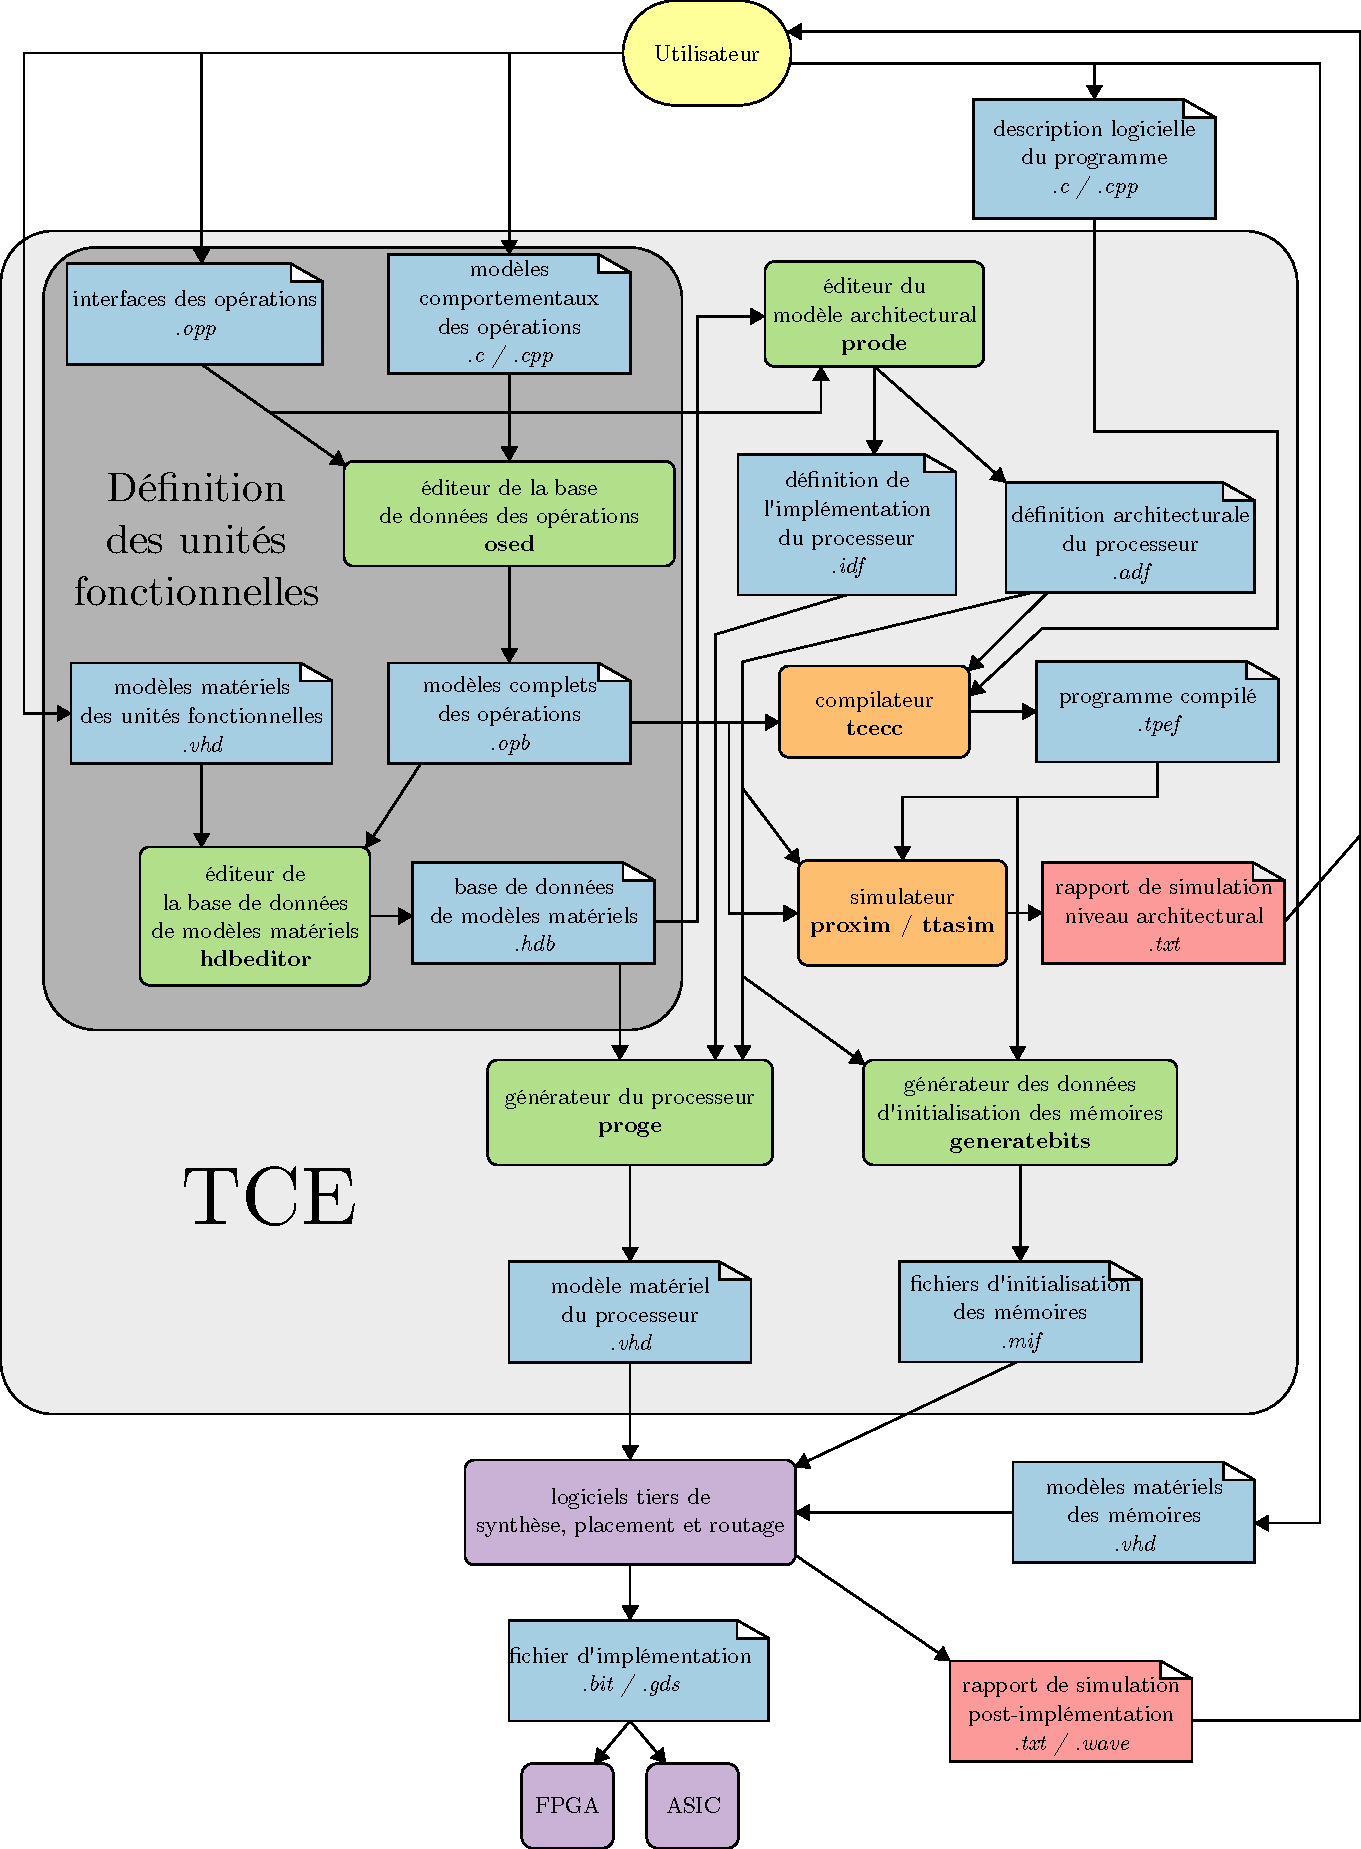
\includegraphics[width=\textwidth]{main/ch4_fig/tce}
\caption{Le flot de conception TCE.}
\label{fig:tce}
\end{figure}
Les modèles matériels des unités fonctionnelles sont décrits en langage VHDL ou Verilog. Un grand nombre de modèles matériels et d'opérations de base sont fournies par la suite logicielle TCE (unités de chargement et de sauvegarde, fichiers de registres, ALU, unités SIMD, ...). Pour créer des unités fonctionnelles spécifiques, l'utilisateur doit décrire l'interface des opérations, leurs modèles comportementaux, et les modèles matériels des unités fonctionnelles dans un langage de description matériel (VHDL ou Verilog). Ces modèles matériels sont réunis dans une base de données de modèles matériels (\textit{.hdb}), éditable et consultable grâce à l'outil \textit{hdbeditor}.
La base de donnée sert au concepteur afin de réutiliser des modèles matériels déjà conçus par lui même ou par d'autres contributeurs.

Le deuxième fichier produit par \textbf{prode} est le fichier de définition de l'implémentation \textit{.idf}. Il relie simplement chaque unité fonctionnelle définie dans le fichier \textit{.adf} à son implémentation matérielle contenue dans la base de donnée de modèles matériels.

\subsubsection{Simulation au niveau architectural.}

Le compilateur (\textbf{tcecc}) utilise le fichier de description architecturale \textit{.adf} et les modèles des opérations afin de compiler la description logicielle du programme écrite par le programmeur. Ce programme est écrit dans un langage haut niveau (C,C++,OpenCL). Un effort particulier a été effectué par les développeurs de l'environnement TCE afin de rendre ce compilateur efficace. Il est basé sur le projet LLVM \cite{lattner_llvm:_2004} et bénéficie à ce titre d'optimisations des premiers niveaux de la chaîne de compilation (analyses lexicale, syntaxique, sémantique et génération du code intermédiaire). Les dernières étapes d'optimisation spécifiques a TTA (dérivation des fichiers de registre, utilisation d'unités fonctionnelles, opérations SIMD) sont réalisées par les développeurs de l'outil TCE.

Le programme compilé peut ensuite être simulé, soit à l'aide d'un outil en ligne de commandes (\textbf{ttasim}), soit par une interface graphique (\textbf{proxim}). Cette simulation permet d'obtenir le nombre de cycles nécessaire à l'exécution de l'intégralité ou d'une partie du programme, et ainsi d'avoir un premier retour sur l'efficacité de l'architecture conçue. D'autres fonctions sont accessibles grâce à ce simulateur. Un profilage peut être réalisé. Il permettra à l'utilisateur de connaître le nombre de cycles d'exécutions pris par chaque fonction et ainsi de connaître les portions du programmes à accélérer prioritairement. Le simulateur donne également des métriques importantes, comme l'engorgement des bus, l'engorgement des sockets ou le taux d'utilisation de chaque opération dans les unités fonctionnelles. Cet ensemble de métriques permet au concepteur d'analyser très finement le fonctionnement du processeur et le déroulement du programme.

\subsubsection{Génération du processeur.}

La dernière étape est la génération du modèle matériel complet du processeur. L'outil de génération du processeur (\textbf{proge}) utilise la base de données des modèles matériels des unités fonctionnelles (fichier \textit{.hdb}) ainsi que les fichiers de description de l'architecture et de l'implémentation du processeur (fichiers \textit{.adf} et \textit{.idf}) afin de créer le modèle complet du processeur. Il intègre donc les différents modèles des unités fonctionnelles, le réseau d'interconnexion, mais également l'unité de contrôle du processeur, visible dans la Figure \ref{fig:tta_example}, qui permet la lecture du programme, stocké dans la mémoire d'instructions.

L'outil \textbf{generatebits} permet quant à lui de générer les contenus d'initialisation des mémoires de données et d'instructions. Les modèles matériels de ces mémoires doivent être fournis par l'utilisateur puiqu'en général, ceux-ci sont dépendants de la cible d'implémentation.

Le modèle matériel du processeur et les modèles des mémoires peuvent ensuite être fournis à un logiciel tiers, pour synthèse et implémentation sur FPGA ou sur ASIC. Les rapports de synthèse ou d'implémentation fournissent alors des métriques concernant la fréquence de fonctionnement, la surface utilisée et la consommation de puissance. Ces métriques peuvent être utilisées par le concepteur afin d'améliorer l'architecture du processeur. Des itérations du flot de conception permettent d'améliorer le processeur jusqu'à l'obtention de performances satisfaisantes.



\section{Transport Triggered Polar Decoders}

\subsection{Architecture du décodeur SC}
\subsection{Description logicielle}
\subsection{Implémentation de l'algorithme SCAN}

\section{Un flot de conception complet}

\subsection{Génération des vecteurs de tests}
\subsection{Cycles de conception}

\section{Expérimentations et mesures}

\subsection{TT-SC}
\subsection{TT-SCAN}


\section*{Conclusion}


